\mychapter{Aspect Ratio}{Aspect Ratio}
When comparing different aspect ratios there are two options, one is to fix the length of the rods and vary the width, and the other is to fix the volume of the particles and vary width and length simultaneously. The first results in relatively stable diffusion coefficients but different gravitational influences, while the latter does the opposite.
\mysection{Constant Length}
With relatively stable diffusion coefficients the largest difference we notice for differing aspect ratios is that there are more collisions for a larger aspect ratio because the small side of a rod is larger. Especially the collisions with the small side lead to locking because the particles can not escape by rotation but only by movement in the opposite direction of the gravitational pull. Hence we can observe for large aspect ratios that most of the movements happen in a shorter time at the start of a simulation and after that the acceptance rate decreases. For small aspect ratios we can see that there is more movement later on because most collisions can be resolved by an energy neutral rotation instead of an energy negative movement. This is also amplified by the differences in the influence of gravitation, since a larger aspect ratio results in a larger volume and hence in a larger gravitational pull. This means that small movements in the opposite direction of the gravitational pull are penalized heavier. We ran a simulation (see~\ref{fig:asp_length}) with a fixed length $l$ for different widths $d$, the number $t^*$ is the number of  last batch of 1000 monte carlo iterations for which more than 1\% of rods in the batch moved or rotated.
\begin{equation}
  \def\arraystretch{1}
  \begin{array}{LCR}
    \text{Material}~~&~\text{Aspect Ratio $\frac{l}{d}$}~&~~t^*\\
    \text{Lithium}&0.16&461\\
    \text{Lithium}&0.08&397\\
    \text{Lithium}&0.04&396\\
    \text{Lithium}&0.02&566\\
    \text{Lithium}&0.01&824\\
    \text{Iron}&0.16&305\\
    \text{Iron}&0.08&523\\
    \text{Iron}&0.04&574\\
    \text{Iron}&0.02&577\\
    \text{Iron}&0.01&1688\\
  \end{array}
\end{equation}
We can see that $t^*$ increases for a smaller aspect ratio, indicating that there are more movements for a smaller aspect ratio. 
\begin{figure}[h]
  \begin{minipage}[t]{0.45\textwidth}
    \fbox{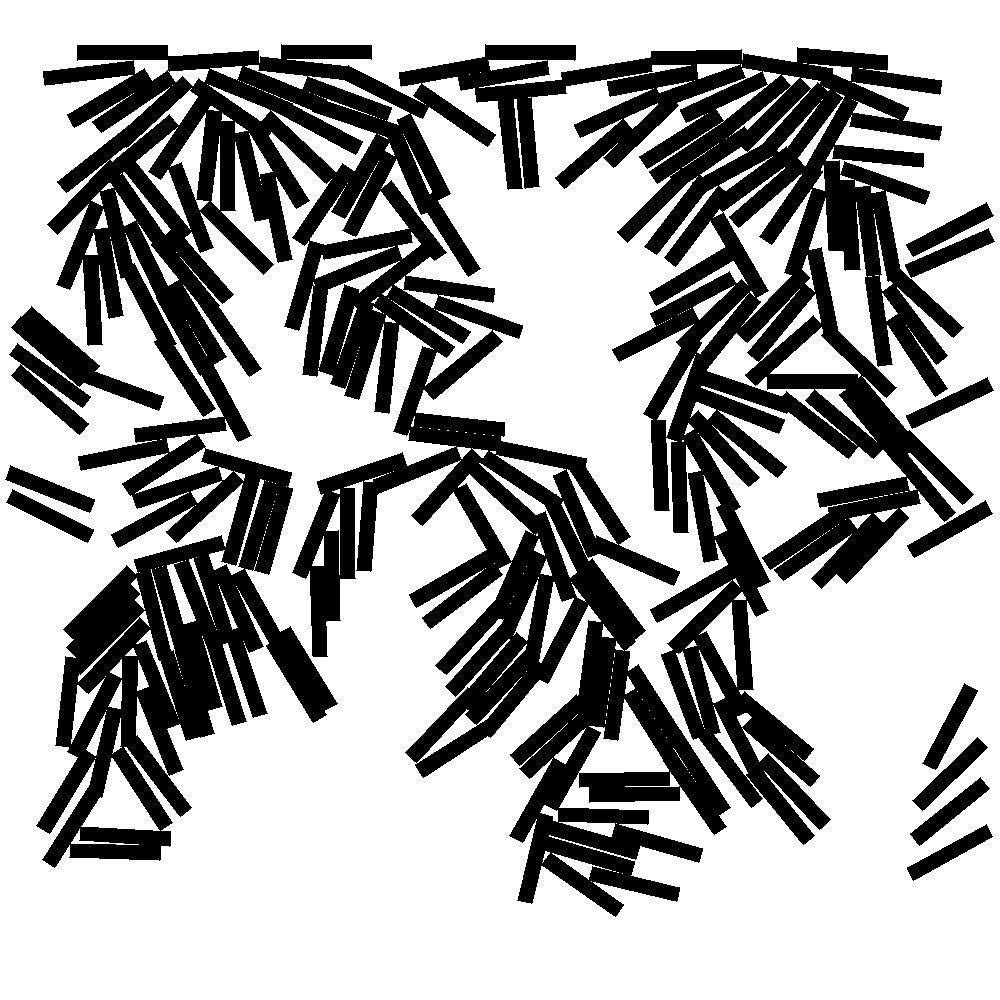
\includegraphics[width=\textwidth]{data/asp_thick.png}}
  \end{minipage}
  \hfill
  \begin{minipage}[t]{0.45\textwidth}
    \fbox{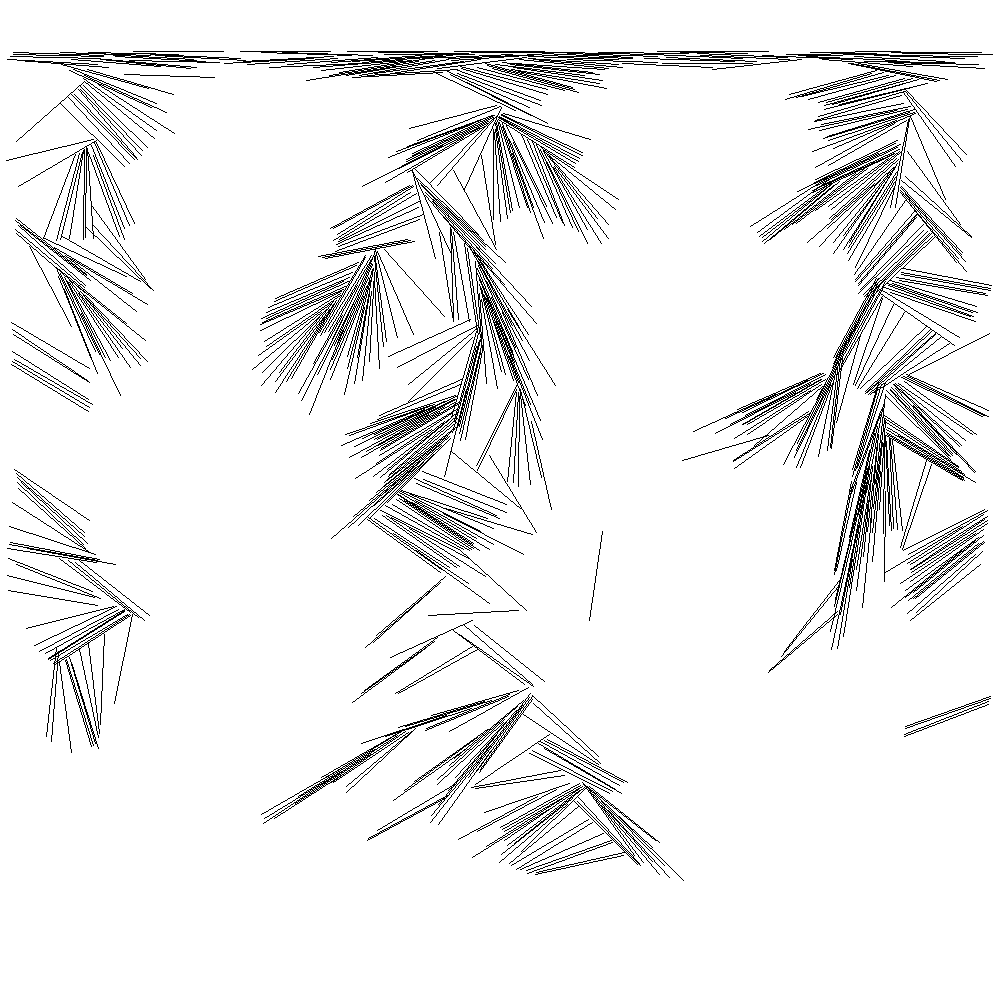
\includegraphics[width=\textwidth]{data/asp_thin.png}}
  \end{minipage}
  \caption{Comparison of lithium rods with equal length and an aspect ratio of 0.16 (left) and 0.01 (right) in water, picture shows end state after 1e7 MC iteration steps.}
  \label{fig:asp_length}
\end{figure}
\mysection{Constant Volume}
To change the aspect ratio $\frac{l}{d}$ by some factor $β$ while keeping the volume $ld^2$ constant, we change the length of the rods to $α^2l$ and the width to $\frac{d}{α}$  for $α= β^{\eb3}$, the resulting changes to the diffusion coefficients are
\begin{equation}
  \begin{array}{RLL}
    D_\|,D_\perp: &α^2\frac{(\ln d  +γ)}{\ln d+ γ  + \ln α}\sim α^2,\\
    D_r:&σ^6\frac{(\ln d  +γ)}{\ln d+ γ  + \ln α}\sim α^6,
  \end{array}
\end{equation}
meaning that the rotational movement disproportionally changes for a changing aspect ratio. This results in a less dense packing for larger aspect ratios, since the rotational movements prevent a close alignment. A dense packing leaves less room for the rods to move and is complemented by a larger surface area of the rods to lead to a lower acceptance rate for small aspect ratios and therefore the opposite result to the last section. We ran a simulation for Iron rods(see~\ref{fig:asp_vol}) with a fixed volume and varying values for $α$, the number of rods was chosen such that the visible cross section of all rods combined was the same for all runs. From the different height of the final stacks, we hence can confirm the differences in packing density. The number $t^*$ is the number of last batch of 1000 monte carlo iterations for which more than 5\% of rods in the batch moved or rotated.
\begin{equation}
  \def\arraystretch{1}
  \begin{array}{LR}\text{Aspect Ratio $\frac{l}{d}$}~&~~t^*\\
    0.017 & 684\\
    0.05& 1075\\
    0.110& 1274\\
    0.169& 1438\\
    0.245& 953\\
    0.4& 2118
  \end{array}
\end{equation}
Apart from the run with aspect ratio 0.245, which could be due to bad luck, this confirms the theory. The different ratios of movement and rotation for different aspect ratios result in a different structure in the final stacks. There always are patches of rods which are aligned in the same direction and at a different angle(almost orthogonal) from neighbouring patches, which can be seen especially good in the third image. These patches have different sizes for the different aspect ratios, for the smallest aspect ratio, there are only two patches and for the largest aspect ratio the patches only consist of few rods.
\begin{figure}[h]
  \begin{minipage}[t]{0.3\textwidth}
    \fbox{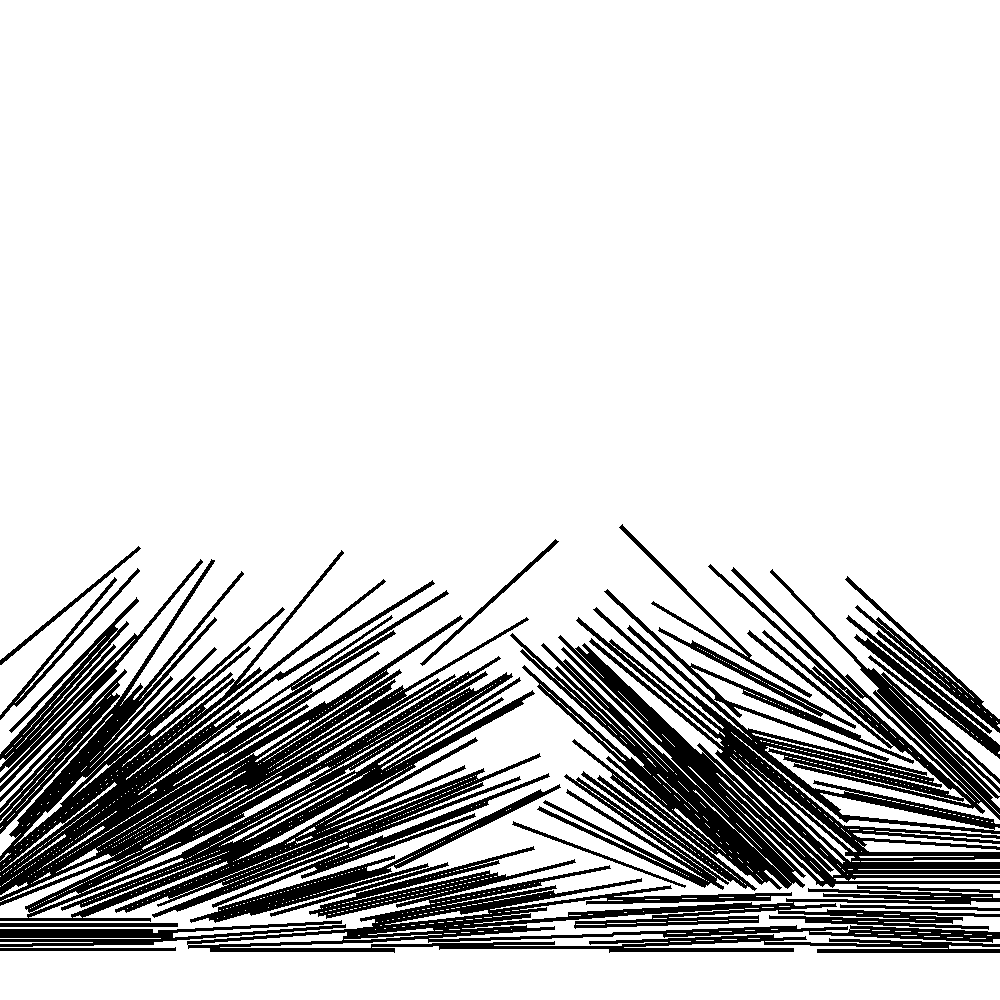
\includegraphics[width=\textwidth]{data/asp_v1.png}}
  \end{minipage}~~~
  \begin{minipage}[t]{0.3\textwidth}
    \fbox{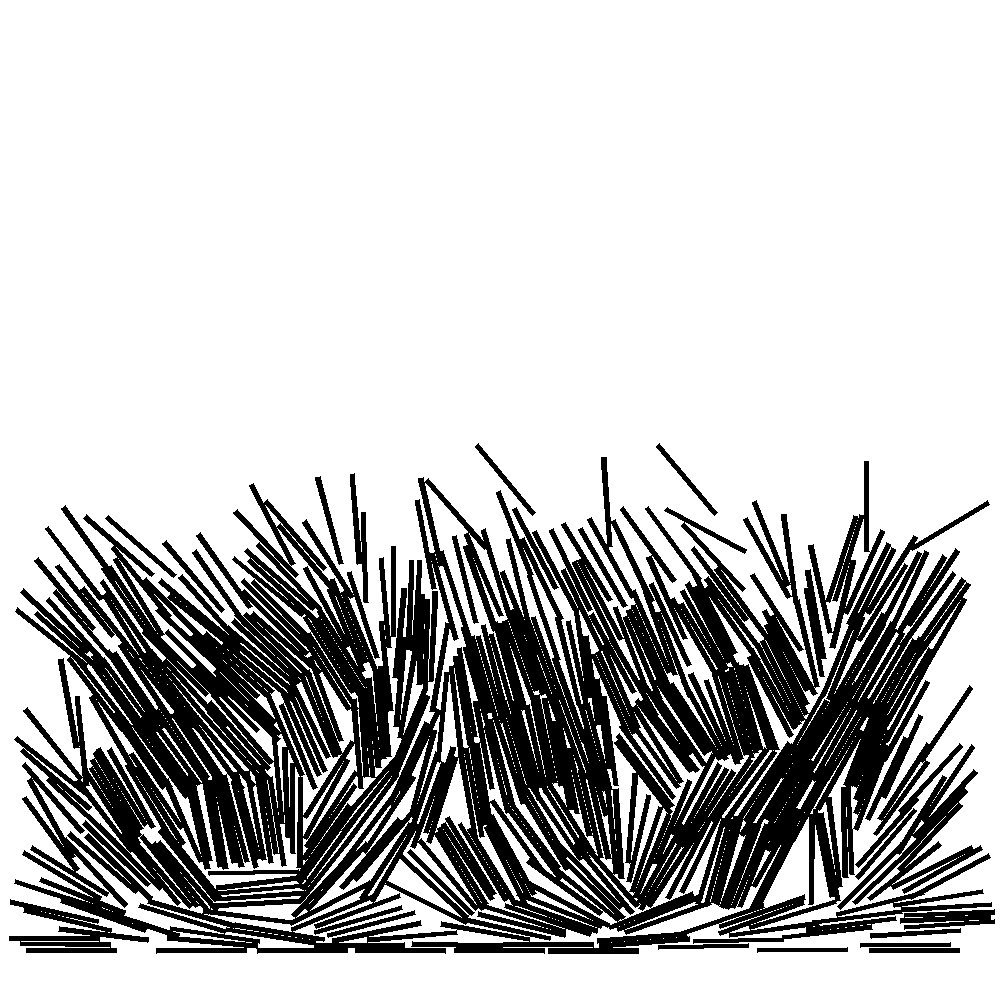
\includegraphics[width=\textwidth]{data/asp_v4.png}}
  \end{minipage}~~~
  \begin{minipage}[t]{0.3\textwidth}
    \fbox{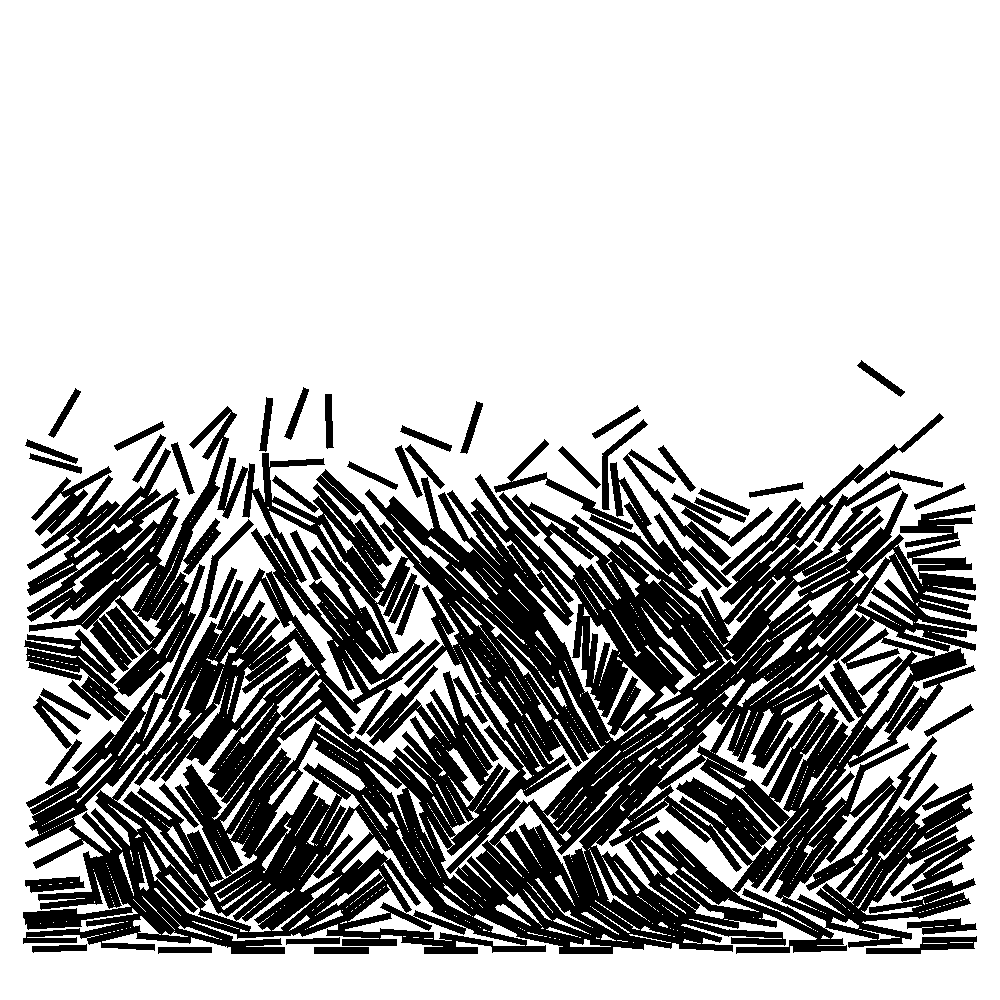
\includegraphics[width=\textwidth]{data/asp_v2.png}}
  \end{minipage}\\\\\\
  \begin{minipage}[t]{0.3\textwidth}
    \fbox{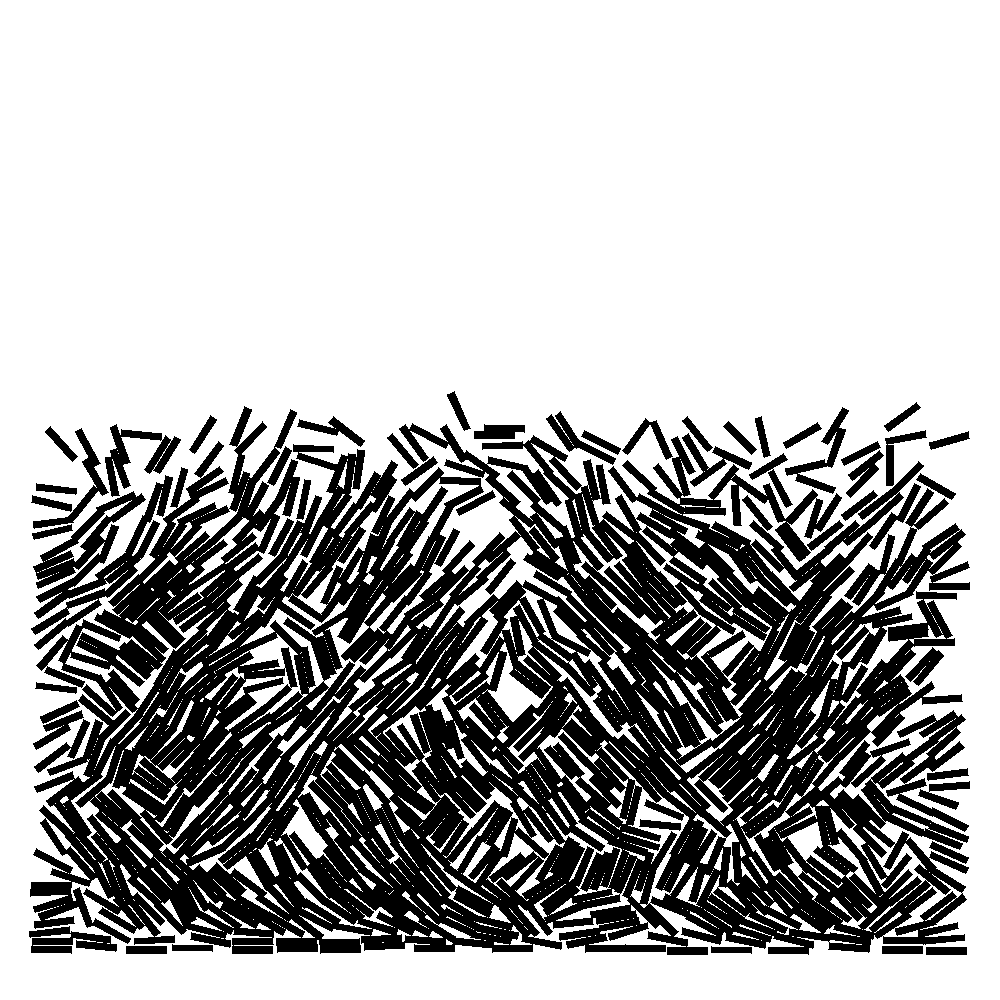
\includegraphics[width=\textwidth]{data/asp_v5.png}}
  \end{minipage}~~~
  \begin{minipage}[t]{0.3\textwidth}
    \fbox{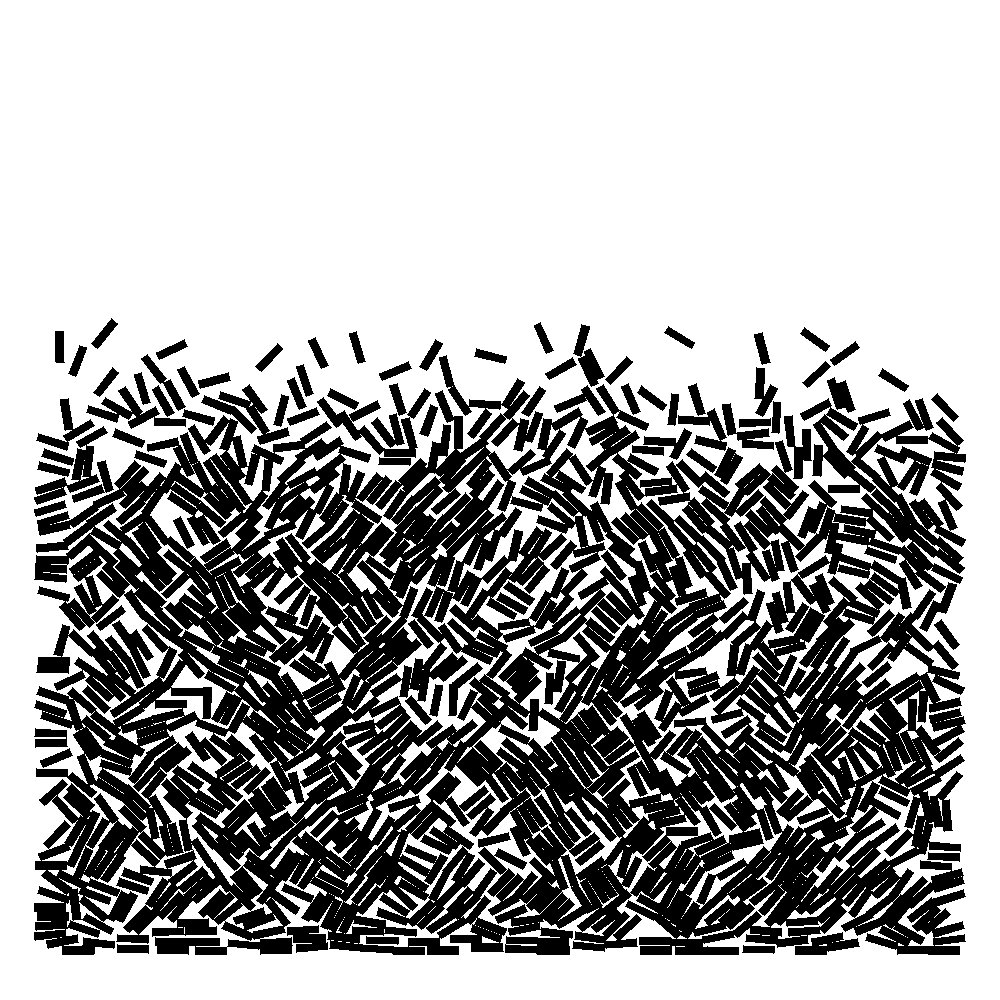
\includegraphics[width=\textwidth]{data/asp_v3.png}}
  \end{minipage}~~~
  \begin{minipage}[t]{0.3\textwidth}
    \fbox{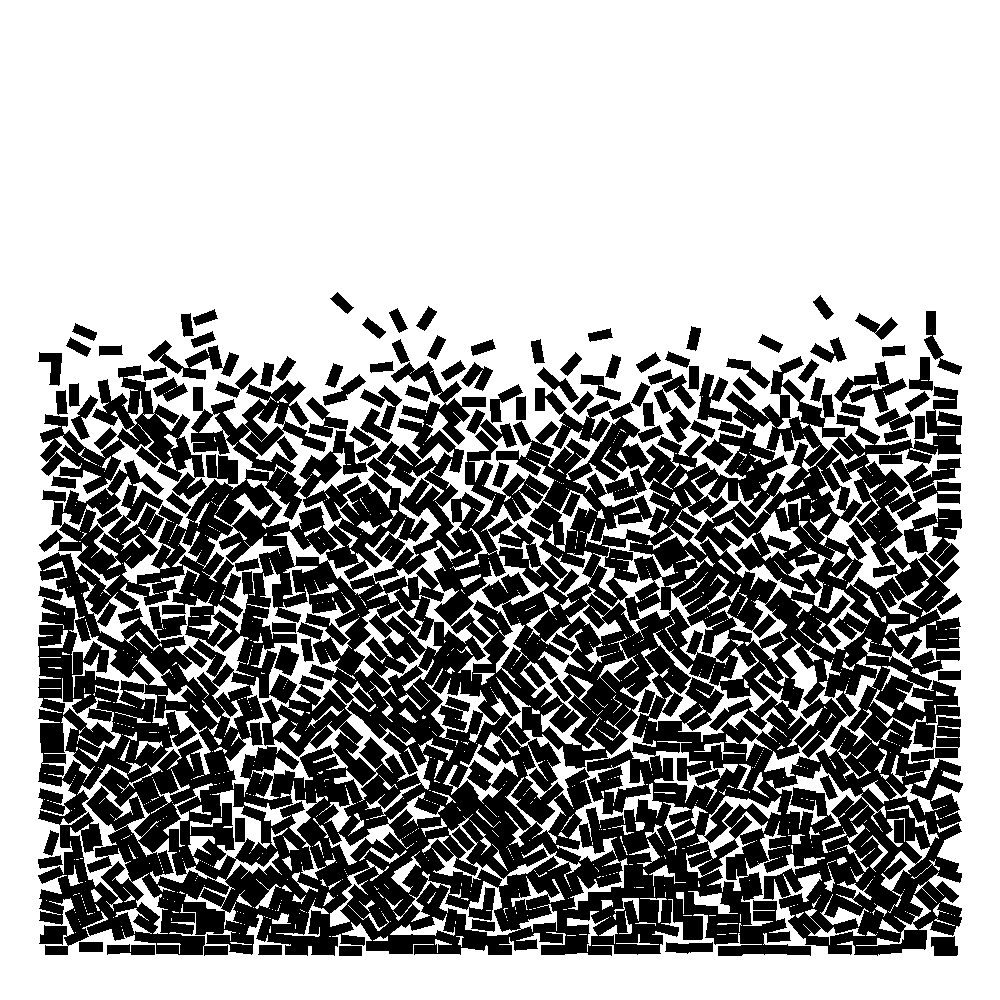
\includegraphics[width=\textwidth]{data/asp_v6.png}}
  \end{minipage}
  \caption{Comparison of iron rods with equal volume and varying aspect ratios from 0.017 (top-left) to  0.4 (bottom-right) in water, picture shows end state after 5e7 MC iteration steps. All simulations were started with an equal total volume of rods}
  \label{fig:asp_vol}
\end{figure}
